\chapter{Thematic Analysis}
\label{appendix-thematic-analysis}

The case studies provided a plethora of findings, these needed to be analysed to establish if common themes emerged. In terms of the six perspectives that had emerged from the case studies, three core groupings were used: for processes, for artefacts, and for analytics tools with the aim of developing the foundations for three chapters of this thesis. Each chapter then discusses the \textit{use} and \textit{improvement} aspects.

There are a wide range of software tools available for thematic analysis. A spreadsheet was the chosen tool, partly so the outputs of the research would be relatively free and easy to share and collaborate on. %Spreadsheet software is ubiquitous both in industry and in research communities and people either already have a software license for a spreadsheet or they can use Google Spreadsheets in a personal capacity free of charge.  

% Notes on many of the various artefacts were summarised in a Google Spreadsheet in support of the analysis and writing up. 
\newthought{Use of Google Spreadsheets to map content to chapters} 
Google's service was chosen as it facilitates a wide range of collaboration without participants needing to pay for software licenses. It also provides useful spreadsheet formulae such as \texttt{FLATTEN}~\footnote{\url{https://support.google.com/docs/answer/10307761?hl=en-GB}} not available in Microsoft Excel at the time of writing.

% The source diagram is in Google Drawing at https://docs.google.com/drawings/d/1A38BJNGKRvdasXVAWRsyaPIaXWPW18618Bti7XwBssI/edit?usp=sharing
\begin{figure}
    \centering
    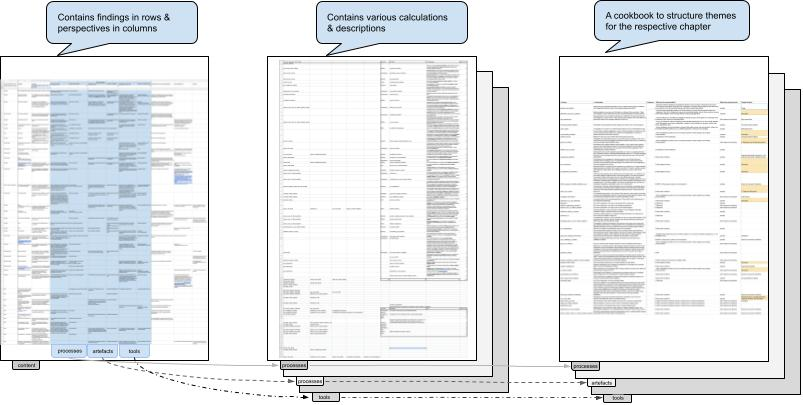
\includegraphics[width=\textwidth]{images/my/Thematic-Analysis-Spreadsheet-Design-28-may-2022a.jpeg}
    \caption{Thematic Analysis Spreadsheet Design}
    \label{fig:thematic-analysis-spreadsheet-design}
\end{figure}

\section{Spreadsheet design and use}
The spreadsheet was designed to take advantage of core spreadsheet features: worksheets for the content, the calculations, the analysis and the mapping, named ranges to identify datasets, and spreadsheet formulae to perform calculations. To make the data easier to process compound-names and full-stops (periods) were used in the theme data cells. And finally, there are two levels of thematic groupings, L2 and L1, where L2 combines L1 themes for reporting purposes.

An artefact can include several themes, where this occurs the themes are listed in the same sell and separated with commas.

\subsection{Worksheets}
The spreadsheet contains three distinct types of worksheet, the first lists artefacts and their primary source(s). The second type includes areas for calculations together with descriptions of all of the respective granular level one (L1) and level two (L2) themes. And the third type is used to identify commonalities for the artefacts that share an L1 theme, their primary focus (research, practice, or both), and a mapping to a section in the respective chapter of this thesis. These three distinct types are illustrated in Figure \ref{fig:thematic-analysis-spreadsheet-design}. 


\subsection{Compound names and full-stops}
Themes incorporate hyphens to join individual words into a compound term, and this term can be processed relatively easily with spreadsheet formulae while also being palatable in \LaTeX ~(unlike underscores that cause \LaTeX ~to incorrectly interpret the underscores as instructions as I discovered, for example \texttt{weaknesses\_in\_dev\_practices} needed each of the \texttt{\_} characters to be prefixed with a backslash \texttt{\textbackslash} in order to print it in the thesis). Examples of themes include: \texttt{use-of-automated-tests} and \texttt{actionable-reports}.

The full-stop character was used in place of an empty cell to enable auto-complete to work down columns that would otherwise have blank cells in some of the row entries. These full-stop characters are accounted for throughout the spreadsheet so they are not counted.


\subsection{Spreadsheet ``named ranges''}
Use of Named Ranges made datasets easier to visualise and identify within the spreadsheet when compared to using hard-coded cell identifiers in spreadsheet formulae. There are individual named ranges for:
\begin{itemize}
    \item process, artefact, and analytics-tool topics,
    \item process, artefact, and analytics-tool themes,
    \item areas used as working storage for formula calculations.
\end{itemize}

The named ranges also use compound names, however rather than using hyphens the first letter of each individual word is capitalised, for example \texttt{ProcessThemes}.%\todo{Replace the remaining hard-coded cell addresses with named ranges and then update this appendix accordingly.}

\subsection{Spreadsheet formulae}
Standard, but not necessarily commonly-used, formulae are used to perform calculations, data expansions, aggregation, and analysis. 

Examples of spreadsheet formulae
{
\footnotesize
\begin{itemize}
    \item Unpack the comma-separated list of themes using the relevant NamedRange, \emph{e.g.} \texttt{=(arrayformula(TRIM(split(ProcessThemes,","))))}
    \item \texttt{=sort(filter(ARRAYFORMULA(UNIQUE(FLATTEN(A2:E113))),ARRAYFORMULA(UNIQUE(FLATTEN(A2:E113))<>"")))}
    \item \texttt{=COUNTA(F3:F44)}
    \item \texttt{=COUNTIF(\$A\$2:\$D\$113, G3)}
    \item Thematic analysis
    \begin{itemize}
        \item \texttt{=(COUNTUNIQUE(arrayformula(TRIM(split(ProcessThemes,",")))))-1} provides a count of all the unique terms found in the themes for processes.
        \item \texttt{=COUNTIF(ProcessThemes, "*improve\_engineering\_practices*")} provides an example of searching for a specific theme amongst the many.
        \item \texttt{=ARRAYFORMULA(FILTER(E5:E156, REGEXMATCH(E5:E156, ".*improve\_engineering\_practices.*")))} finds the other terms combined with the search term.
    \end{itemize}
    
    \item \texttt{="Source project|tool ("\&COUNTA(A5:A998)\&")"}
    
    \item \texttt{="Processes ("\&COUNTA(D5:D1000)\&")"}, ="Artefacts ("\&COUNTA(F5:F1000)\&")", ="Analytics Tools ("\&COUNTA(H5:H1000)\&")"
    \item \texttt{=sort(UNIQUE(F3:F37))}
    \item \texttt{=sum(I3:I44)}
    \item \texttt{\href{https://support.google.com/docs/answer/3094098?hl=en-GB}{=RANK}(G3, AnalyticsToolsL1Counts)} Ranks the frequency of the L1 themes for any of the three chapters the present the findings.
\end{itemize}
}

\subsection{Inclusion criteria for a chapter}
The top-ranked L1 themes were selected for the \href{chapter-tools-and-their-artefacts}{Analytics Tools} chapter as they have the strongest base of evidence. These are augmented by key topics even if they do not rank as highly as the top \emph{nn}; and additional L1 themes are also included within the thesis when it was germane to do so, for instance to support a point or provide additional evidence. 
